\section[I componenti elettronici]{I componenti elettronici}
\label{sec:electronics}
\sectionframe{images/covers/cover_architecture.jpeg}{I componenti elettronici}


\begin{frame}
	\frametitle{Il computer}
	
	\begin{block}{I componenti elettronici di un computer}
		I componenti elettronici che formano un computer possono essere sintetizzati in due categorie principali:
		\begin{itemize}
			\item \textbf{porte logiche} (per realizzare le quali si utilizzano i \textbf{transistor})
			\item \textbf{generatori di segnali}
		\end{itemize}
		
		Approfondiamoli nelle slides successive.
	\end{block}
\end{frame}



\subsection[I transistor]{I transistor}
\begin{frame}
	\frametitle{I transistor}
	
	\begin{columns}			
		\column{0.6\linewidth}
		\begin{block}{I microprocessori e i microcontrollori}
			I microprocessori e i microcontrollori sono componenti chiave dei computer e dei dispositivi elettronici in quanto ne costituiscono il "cervello".\\~\\
			Uno dei componenti elettronici più importanti all'interno di questi sono i \textbf{transistor}, utilizzati al loro interno per:
			\begin{itemize}
				\item creare \textbf{circuiti logici}, utilizzati per eseguire calcoli di logica e aritmetica e prendere decisioni,
				\item \textbf{memorizzare informazioni} al loro interno
			\end{itemize} 
		\end{block}
		
		\column{0.4\linewidth}
		\begin{figure}[!htbp]
			\centering 
			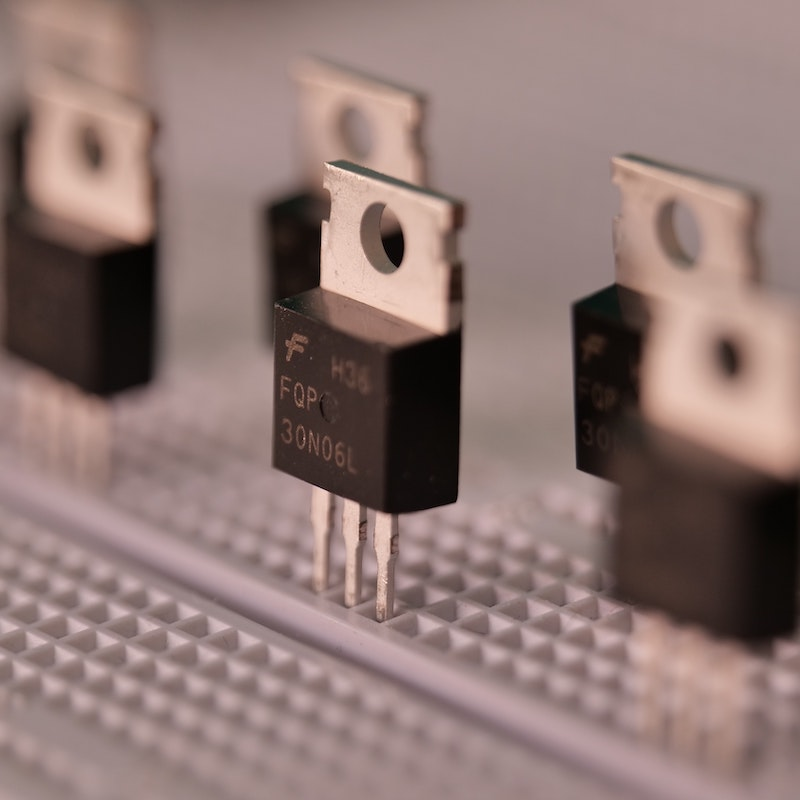
\includegraphics[width=0.95\linewidth]{images/2_elettronica/transistor.jpg}
			\caption{Transistors}
			\label{fig:electronics_transistors}
		\end{figure}		
	\end{columns}
	
\end{frame}




\begin{frame}
	\frametitle{I Transistor}
	
	\begin{columns}			
		\column{0.6\linewidth}
		\begin{block}{I Transistor}
			I transistor sono componenti elettronici utilizzati in molti circuiti elettronici in quanto permettono di \textbf{amplificare} o \textbf{interrompere} un \textbf{segnale elettrico}.
		\end{block}
		
		\begin{block}{16 Dic 1947, Bardeen, Brattain e Shockley riuscirono a creare il primo transistor}
			all'interno degli \textbf{AT\&T Bell Laboratories} (un centro di ricerca e sviluppo, attualmente di proprietà di Nokia) da allora sono diventati un componente chiave dell'elettronica.
		\end{block}
		
		\column{0.4\linewidth}
		\begin{figure}[!htbp]
			\centering 
			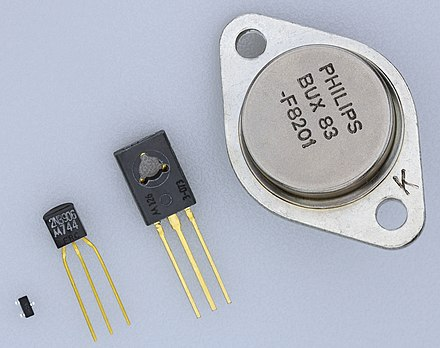
\includegraphics[width=0.95\linewidth]{images/2_elettronica/transistors.jpg}
			\caption{Confronto tra diversi transistor BJT, da sinistra a destra: SOT-23, TO-92, TO-126, TO-3}
		\end{figure}		
	\end{columns}
	
\end{frame}



\begin{frame}
	\frametitle{I Transistor}
	
	\begin{columns}			
		\column{0.6\linewidth}
		\begin{block}{Il Nobel}
			Il transistor doveva inizialmente servire a \textbf{migliorare le comunicazioni} tra il continente americano e quello europeo oggi lo troviamo impiegato nei campi più disparati (informatica, telefonia, smart-car, radio, ...).\\~\\
			Nel \textbf{1956} i tre scienziati statunitensi hanno ricevuto il \textbf{Premio Nobel per la Fisica} per gli studi condotti all'interno dei laboratori di ricerca e sviluppo dell'AT\&T: in appena 9 anni il transistor è diventato una delle componenti hardware più importanti e utilizzate in ambito elettronico.
		\end{block}
		
		\column{0.4\linewidth}
		\begin{figure}[!htbp]
			\centering 
			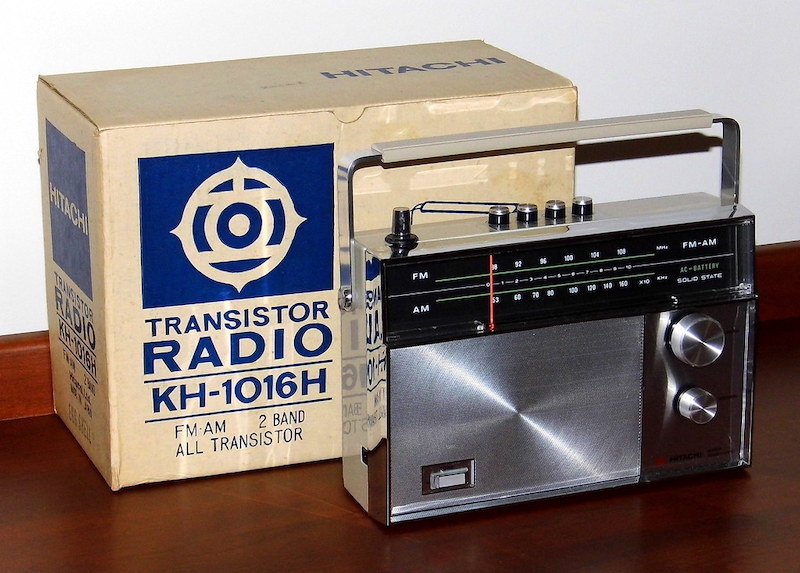
\includegraphics[width=0.95\linewidth]{images/2_elettronica/radio_transistors.jpeg}
			\caption{I transistor sono usati nelle radio sia per amplificare il segnale radiofonico   ricevuto dall'antenna che per il circuito di sintonizzazione utilizzato per selezionare la frequenza del segnale radiofonico.}
		\end{figure}		
	\end{columns}
	
\end{frame}


\subsubsection[La capacità di integrazione]{La capacità di integrazione}
\begin{frame}
	\frametitle{La capacità di integrazione}
	
	\begin{block}{La capacità di integrazione}
		Si definisce \textbf{capacità di integrazione} la misura di quanti transistor sono realizzati all'interno di un unico chip integrato:
		\begin{itemize}
			\item SSI (Small Scale Integration): $\qquad\quad\,$ < 100 transistor
			\item MSI (Medium Scale Integration): $\quad\;\;\:$ < 1000 transistor
			\item LSI (Large Scale of Integration): $\quad\;\;\,\,\,$ < 10.000 transistor
			\item VLSI (Very Large Scale Integration): $\,\,$ < 100.000 transistor
			\item ULSI (Ultra Large Scale Integration): $\,$ > 100.000 transistor
		\end{itemize}
		
	\end{block}
	
\end{frame}


\subsubsection[La legge di Moore]{La legge di Moore}
\begin{frame}
	\frametitle{La legge di Moore}
	
	\begin{block}{$\qquad$La legge di Moore}
		\begin{quote}
			La complessità di un microcircuito, misurata ad esempio tramite il numero di transistor per chip, raddoppia ogni 18 mesi (e quadruplica quindi ogni 3 anni).
		\end{quote}		
	\end{block}
	
	\pause
	
	\begin{block}{La storia dietro l'enunciato}
		Nel 1965 \textbf{Gordon Moore} (cofondatore di Intel con Robert Noyce) ipotizzò che il numero di transistori nei microprocessori sarebbe raddoppiato ogni \textbf{12 mesi} circa. 	La legge viene riformulata alla fine degli anni ottanta ed elaborata nella sua forma definitiva, ovvero che il numero di transistori nei processori raddoppia ogni \textbf{18 mesi}.\\
		Questa legge è diventata il metro e l'obiettivo di tutte le aziende che operano nel settore come Intel e AMD.
	\end{block}
	
\end{frame}


\begin{frame}
%	\frametitle{La legge di Moore}
	
%	\begin{block}{Evoluzione del numero di transistors nei microprocessori 1971-2008}
		\begin{figure}[!htbp]
			\centering
			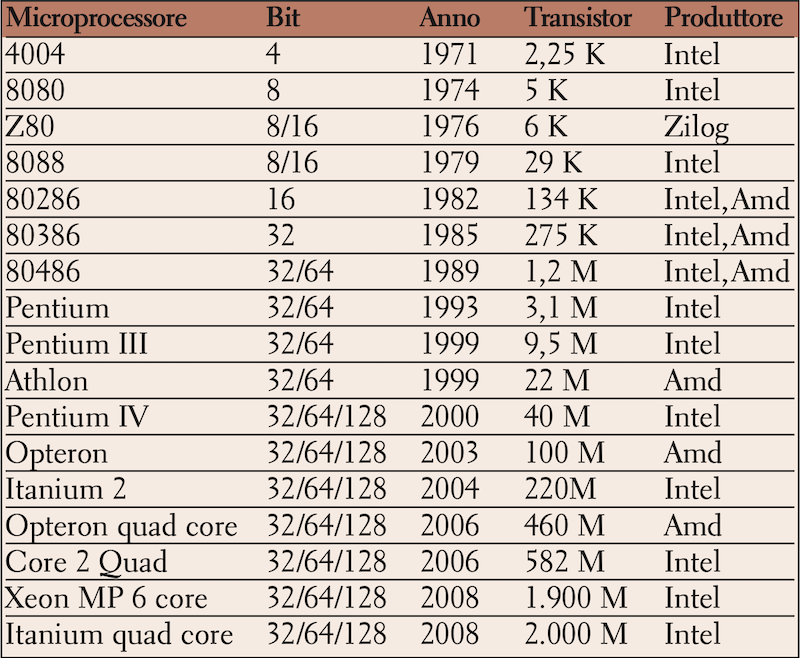
\includegraphics[width=0.7\linewidth]{images/2_elettronica/moore.png}
			\caption{Evoluzione del numero di transistors nei microprocessori 1971-2008}
		\end{figure}
%	\end{block}

	
	
\end{frame}


\begin{frame}
%	\frametitle{La legge di Moore}
	
	\begin{figure}[!htbp]
		\centering 
		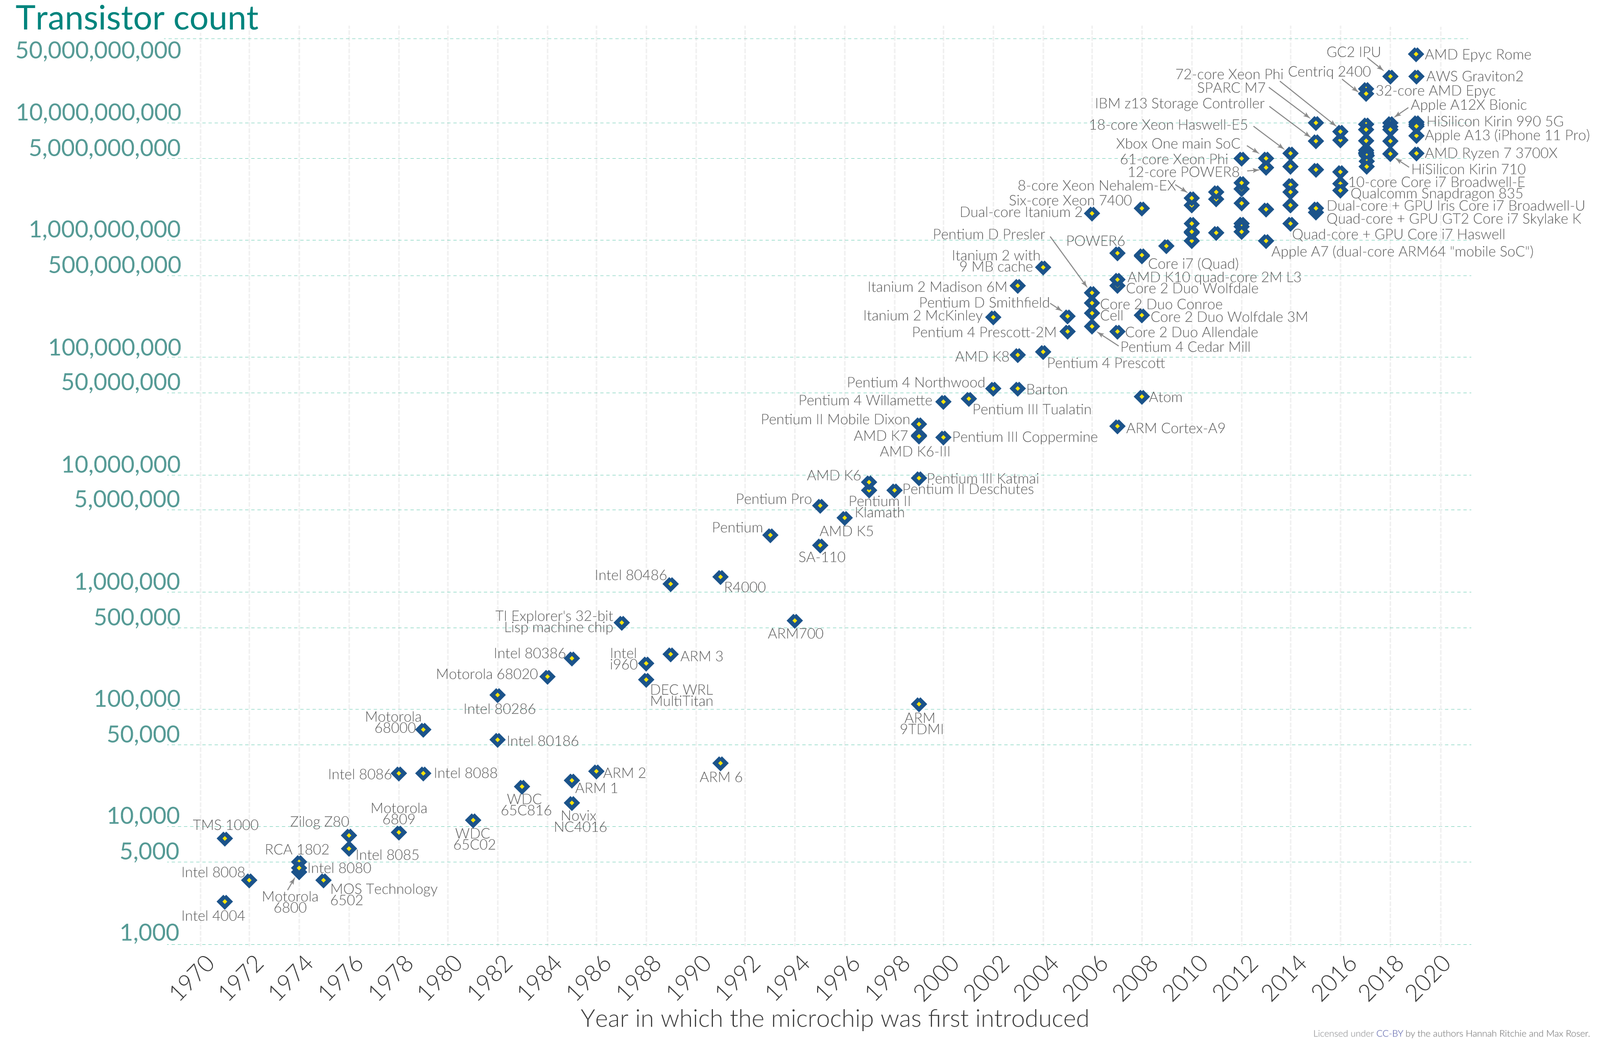
\includegraphics[width=1.02\linewidth]{images/2_elettronica/Moore's_Law_Transistor_Count_1970-2020.png}
%		\caption{}
		\label{fig:electronics_moorelaw}	
	\end{figure}
	
\end{frame}



\subsection[Le porte logiche]{Le porte logiche}
\begin{frame}
	\frametitle{Le porte logiche}
	
	\begin{block}{Le porte logiche}
		Grazie ai transistor è possibile realizzare dei circuiti logici (vedi \hyperlink{fig:electronics_transistors}{pag. \pageref{fig:electronics_transistors}}).\\
		Le \textbf{porte logiche} sono dei circuiti elettronici elementari in grado di svolgere le operazioni logiche dell'algebra booleana basata sui valori logici:
		\begin{itemize}
			\item \textbf{TRUE} oppure \textbf{1}: passaggio di corrente (tensione alta)
			\item \textbf{FALSE} oppure \textbf{0}: non passaggio di corrente (tensione bassa)
		\end{itemize}
	\end{block}
	$\qquad\qquad\qquad\qquad\:$Le tre porte logiche principali sono:
	
	\begin{columns}
		\column{0.33\linewidth}
		\begin{figure}[!htbp]
			\centering 
			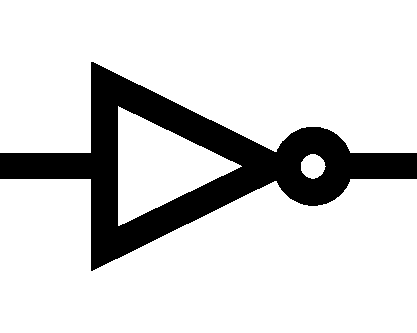
\includegraphics[width=0.5\linewidth]{images/2_elettronica/logic_gate_not.pdf}
			\caption{Porta logica \textit{NOT}}
		\end{figure}
		
		\column{0.33\linewidth}
		\begin{figure}[!htbp]
			\centering 
			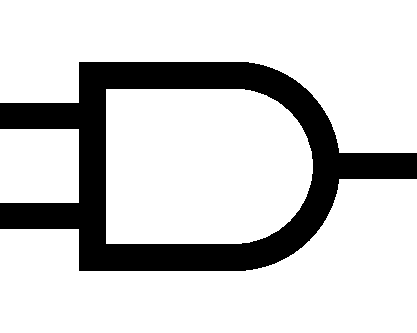
\includegraphics[width=0.5\linewidth]{images/2_elettronica/logic_gate_and.pdf}
			\caption{Porta logica \textit{AND}}
		\end{figure} 
		
		\column{0.33\linewidth}
		\begin{figure}[!htbp] 
			\centering 
			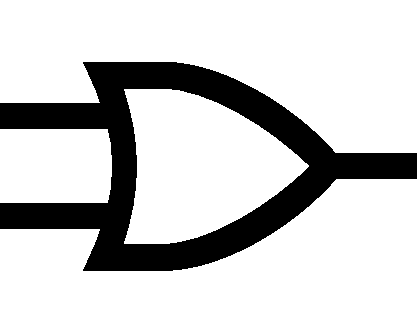
\includegraphics[width=0.5\linewidth]{images/2_elettronica/logic_gate_or.pdf}
			\caption{Porta logica \textit{OR}}
		\end{figure}
		
	\end{columns}
	
\end{frame}


\subsubsection[La porta logica NOT]{La porta logica NOT}
\begin{frame}
	\frametitle{La porta logica NOT}
	
	
	\begin{block}{La porta logica NOT}
		è la porta logica che implementa la \textbf{negazione logica}.\\Tale dispositivo restituisce il \textbf{valore negato del livello logico} in ingresso.
	\end{block}

	\begin{columns}
		\column{0.3\linewidth}
		\begin{figure}[!htbp]
			\centering 
			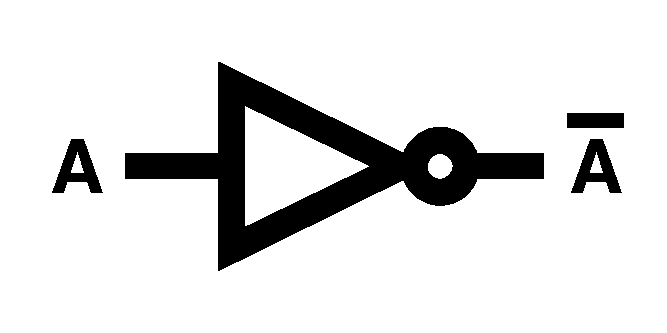
\includegraphics[width=0.9\linewidth]{images/2_elettronica/logic_gate_not_a.pdf}
			\caption{Icona}
		\end{figure}
		
		\column{0.4\linewidth}
		\begin{table}[]
		\begin{tabular}{|
		>{\columncolor[HTML]{C0C0C0}}c |c|}
		\hline
		\cellcolor[HTML]{EFEFEF}\textbf{A} & \cellcolor[HTML]{EFEFEF}\textbf{NOT A} \\ \hline
		0                                  & 1                                      \\ \hline
		1                                  & 0                                      \\ \hline
		\end{tabular}
		\caption{Tabella di verità}
		\end{table}
		
		\column{0.3\linewidth}
		\begin{figure}[!htbp]
			\centering 
			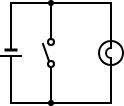
\includegraphics[width=0.85\linewidth]{images/2_elettronica/logic_gate_circuit_not.png}
			\caption{Circuito}
		\end{figure}
		
	\end{columns}
	
\end{frame}



\subsubsection[La porta logica AND]{La porta logica AND}
\begin{frame}
	\frametitle{La porta logica AND}
	
	
	\begin{block}{La porta logica AND}
		è la porta logica che implementa la \textbf{congiunzione logica}.\\
		L'uscità è alta (a 1) solo se entrambi i valori di input A e B sono alti, in tutti gli altri casi l'uscita è bassa (a 0).\\
		In altre parole, la funzione AND corrisponde a trovare il \textbf{minimo} tra due cifre binarie (o a un \textbf{prodotto} tra due cifre binarie).
	\end{block}

	\begin{columns}
		\column{0.3\linewidth}
		\begin{figure}[!htbp]
			\centering 
			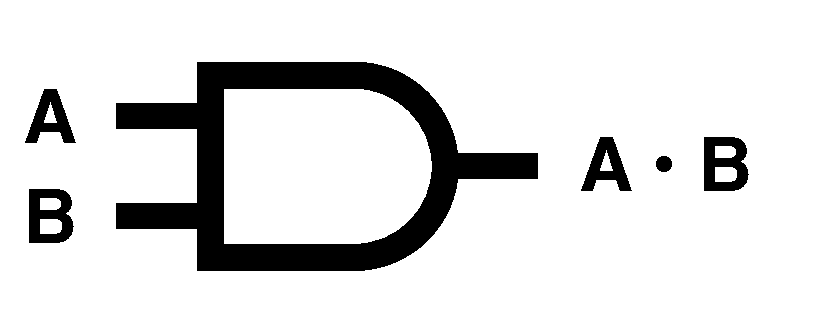
\includegraphics[width=1.0\linewidth]{images/2_elettronica/logic_gate_and_ab.pdf}
			\caption{Icona}
		\end{figure}
		
		\column{0.4\linewidth}
		\begin{table}[]
		\begin{tabular}{|
		>{\columncolor[HTML]{C0C0C0}}c |
		>{\columncolor[HTML]{C0C0C0}}c |c|}
		\hline
		\cellcolor[HTML]{EFEFEF}\textbf{A} & \cellcolor[HTML]{EFEFEF}\textbf{B} & \cellcolor[HTML]{EFEFEF}\textbf{A $\bullet$ B} \\ \hline
		0                                  & 0                         & 0                                    \\ \hline
		0                                  & 1                         & 0                                    \\ \hline
		1                                  & 0                         & 0                                    \\ \hline
		1                                  & 1                         & 1                                    \\ \hline
		\end{tabular}
		\caption{Tabella di verità}
		\end{table}
		
		\column{0.3\linewidth}
		\begin{figure}[!htbp]
			\centering 
			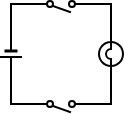
\includegraphics[width=0.85\linewidth]{images/2_elettronica/logic_gate_circuit_and.png}
			\caption{Circuito}
		\end{figure}
		
	\end{columns}
	
\end{frame}


\subsubsection[La porta logica OR]{La porta logica OR}
\begin{frame}
	\frametitle{La porta logica OR}
	
	
	\begin{block}{La porta logica OR}
		è la porta logica digitale che implementa la \textbf{disgiunzione logica}.\\
		L'uscità è bassa (a 0) solo se entrambi i valori di input A e B sono bassi, in tutti gli altri casi l'uscita è alta (a 1).\\
		In altre parole, la funzione OR corrisponde a trovare il \textbf{massimo} tra due cifre binarie.
	\end{block}

	\begin{columns}
		\column{0.3\linewidth}
		\begin{figure}[!htbp]
			\centering 
			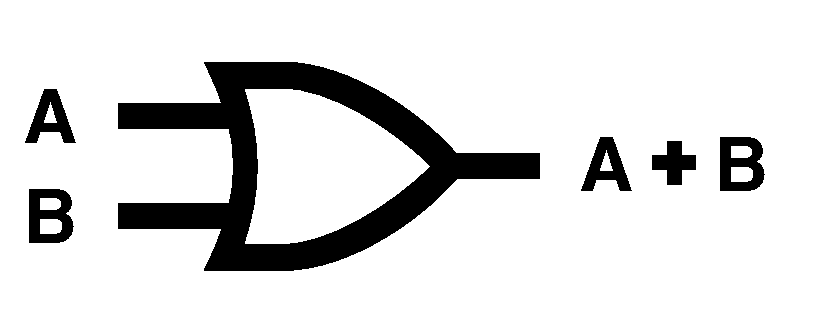
\includegraphics[width=1.0\linewidth]{images/2_elettronica/logic_gate_or_ab.pdf}
			\caption{Icona}
		\end{figure}
		
		\column{0.4\linewidth}
		\begin{table}[]
		\begin{tabular}{|
		>{\columncolor[HTML]{C0C0C0}}c |
		>{\columncolor[HTML]{C0C0C0}}c |c|}
		\hline
		\cellcolor[HTML]{EFEFEF}\textbf{A} & \cellcolor[HTML]{EFEFEF}\textbf{B} & \cellcolor[HTML]{EFEFEF}\textbf{A $+$ B} \\ \hline
		0                                  & 0                         & 0                                    \\ \hline
		0                                  & 1                         & 1                                    \\ \hline
		1                                  & 0                         & 1                                    \\ \hline
		1                                  & 1                         & 1                                    \\ \hline
		\end{tabular}
		\caption{Tabella di verità}
		\end{table}
		
		\column{0.3\linewidth}
		\begin{figure}[!htbp]
			\centering 
			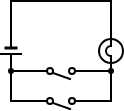
\includegraphics[width=0.85\linewidth]{images/2_elettronica/logic_gate_circuit_or.png}
			\caption{Circuito}
		\end{figure}
		
	\end{columns}
	
\end{frame}



\subsubsection[Altre porte logiche: XOR, NAND, NOR, XNOR]{Altre porte logiche: XOR, NAND, NOR, XNOR}
\begin{frame}
	\frametitle{Altre porte logiche: XOR, NAND, NOR, XNOR}
	
	
	\begin{block}{Altre porte logiche: XOR, NAND, NOR, XNOR}
		Esistono altre porte logiche oltre a NOT, AND e OR.\\
		Tra le più importanti citiamo:
		\begin{itemize}
			\item XOR: l'OR esclusivo
			\item NAND: l'AND negato
			\item NOR: l'OR negato
			\item XNOR: lo XOR negato
		\end{itemize}
	\end{block}
	
\end{frame}


\subsubsection[Tabelle di verità: AND, OR, XOR, NAND, NOR e XNOR]{Tabelle di verità: AND, OR, XOR, NAND, NOR e XNOR}
\begin{frame}
	\frametitle{Tabelle di verità: AND, OR, XOR, NAND, NOR e XNOR}

	\begin{figure}[!htbp]
		\centering 
		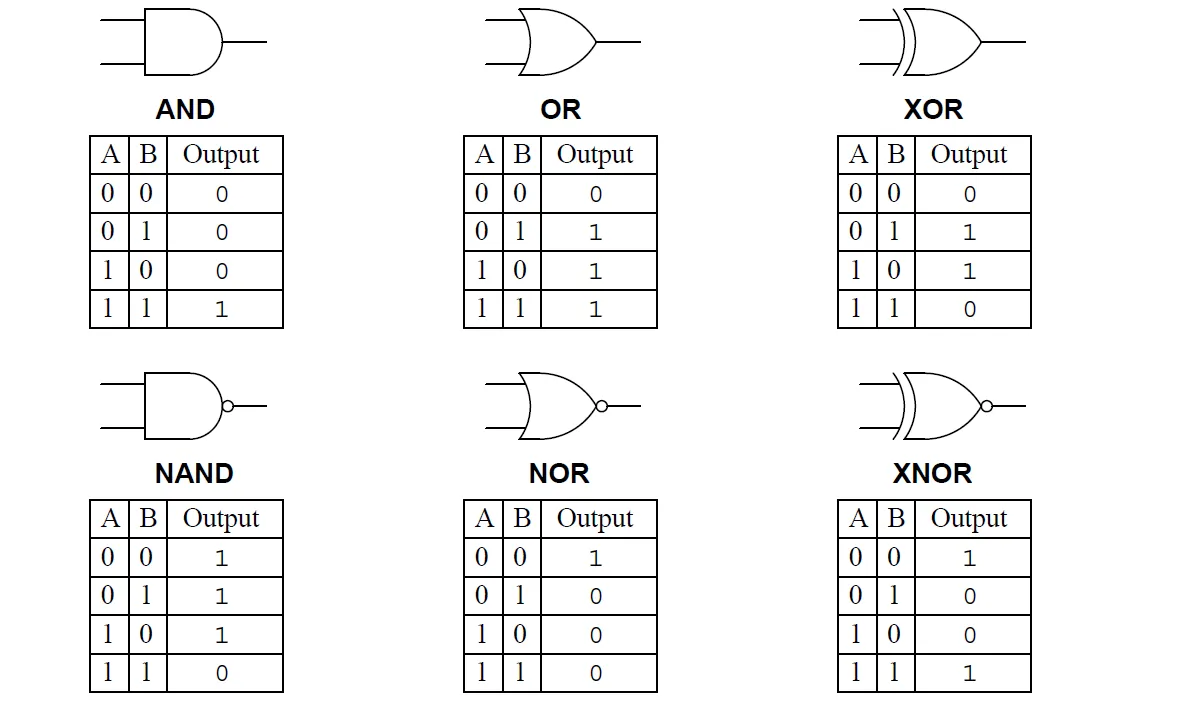
\includegraphics[width=1.0\linewidth]{images/2_elettronica/logic_gates_truthtables.png}
%		\caption{}
	\end{figure}
	
\end{frame}


\subsubsection[Le leggi di De Morgan]{Le leggi di De Morgan}
\begin{frame}
	\frametitle{Le leggi di De Morgan}

	\begin{block}{Le leggi di De Morgan}
		Le \textbf{leggi di De Morgan}, o teoremi di De Morgan, sono relativi alla logica booleana e stabiliscono relazioni di equivalenza tra gli operatori di congiunzione e disgiunzione logica.\\ \vspace{0.8em}
		
		\begin{enumerate}
			\item $\overline{A \cdot B} = \overline A + \overline B$\\
			siccome è possibile riscriverla così: $A \cdot B = \overline{\overline A + \overline B}$ deduciamo che possiamo ottenere un AND combinando adeguatamente NOT e OR.
			\item $\overline{A + B} = \overline {A} \cdot \overline {B}$	\\
			siccome è possibile riscriverla così: $A + B = \overline{\overline {A} \cdot \overline {B}}$
			deduciamo che possiamo ottenere un OR combinando adeguatamente NOT e AND.
		\end{enumerate}
		
	\end{block}
	
\end{frame}


\begin{frame}
	\frametitle{Le leggi di De Morgan: circuiti equivalenti}

	\begin{figure}[!htbp]
		\centering 
		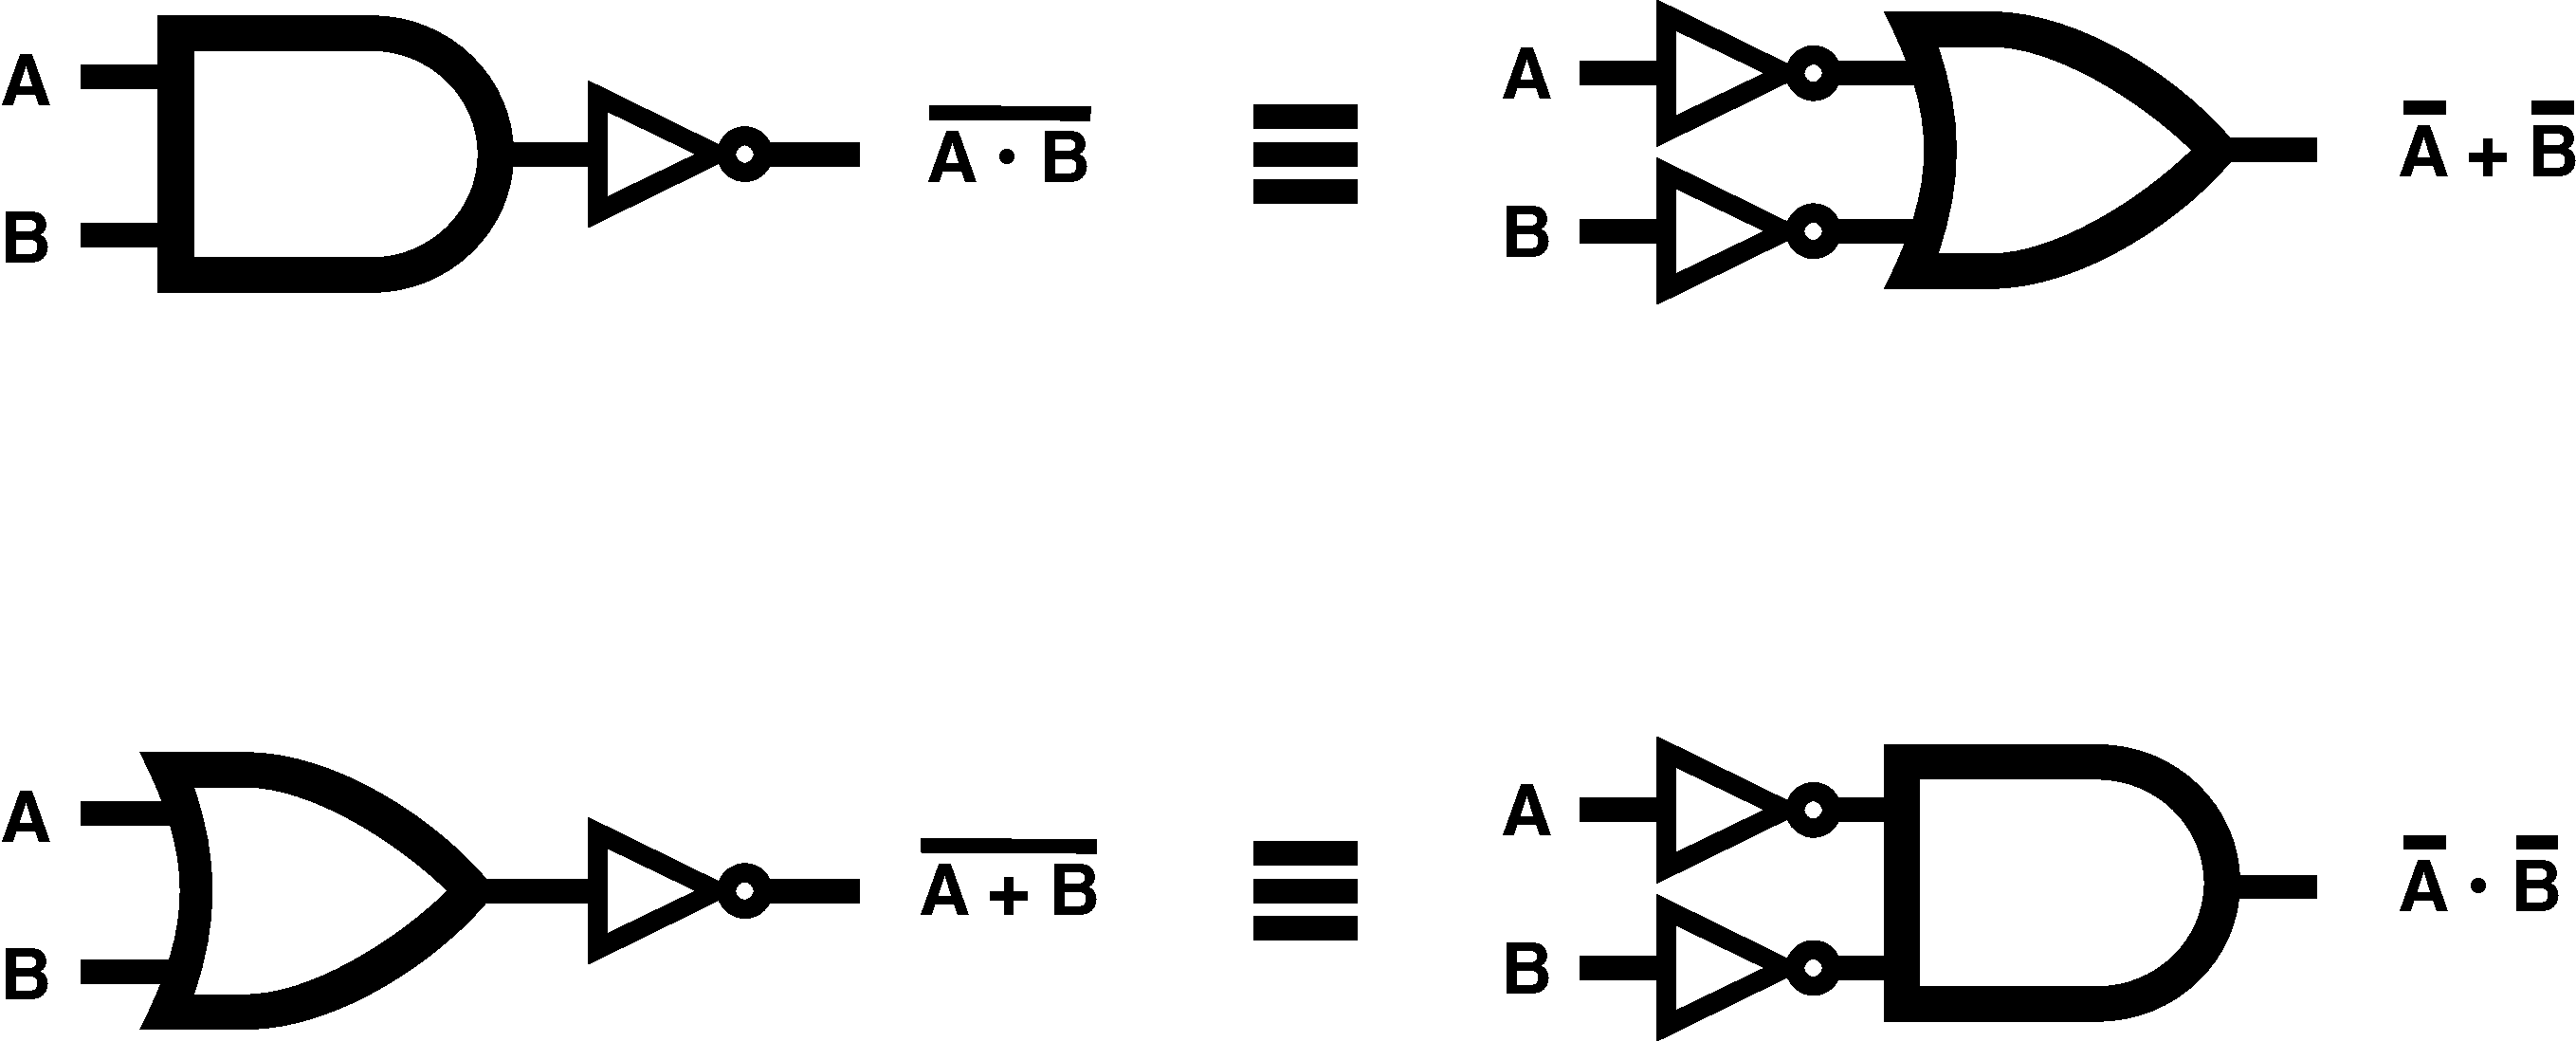
\includegraphics[width=0.8\linewidth]{images/2_elettronica/demorgan_1.pdf}
%		\caption{}
	\end{figure}
	
\end{frame}

\begin{frame}
	\frametitle{Le leggi di De Morgan: circuiti equivalenti (nega a dx e sx)}
	
	\begin{figure}[!htbp]
		\centering 
		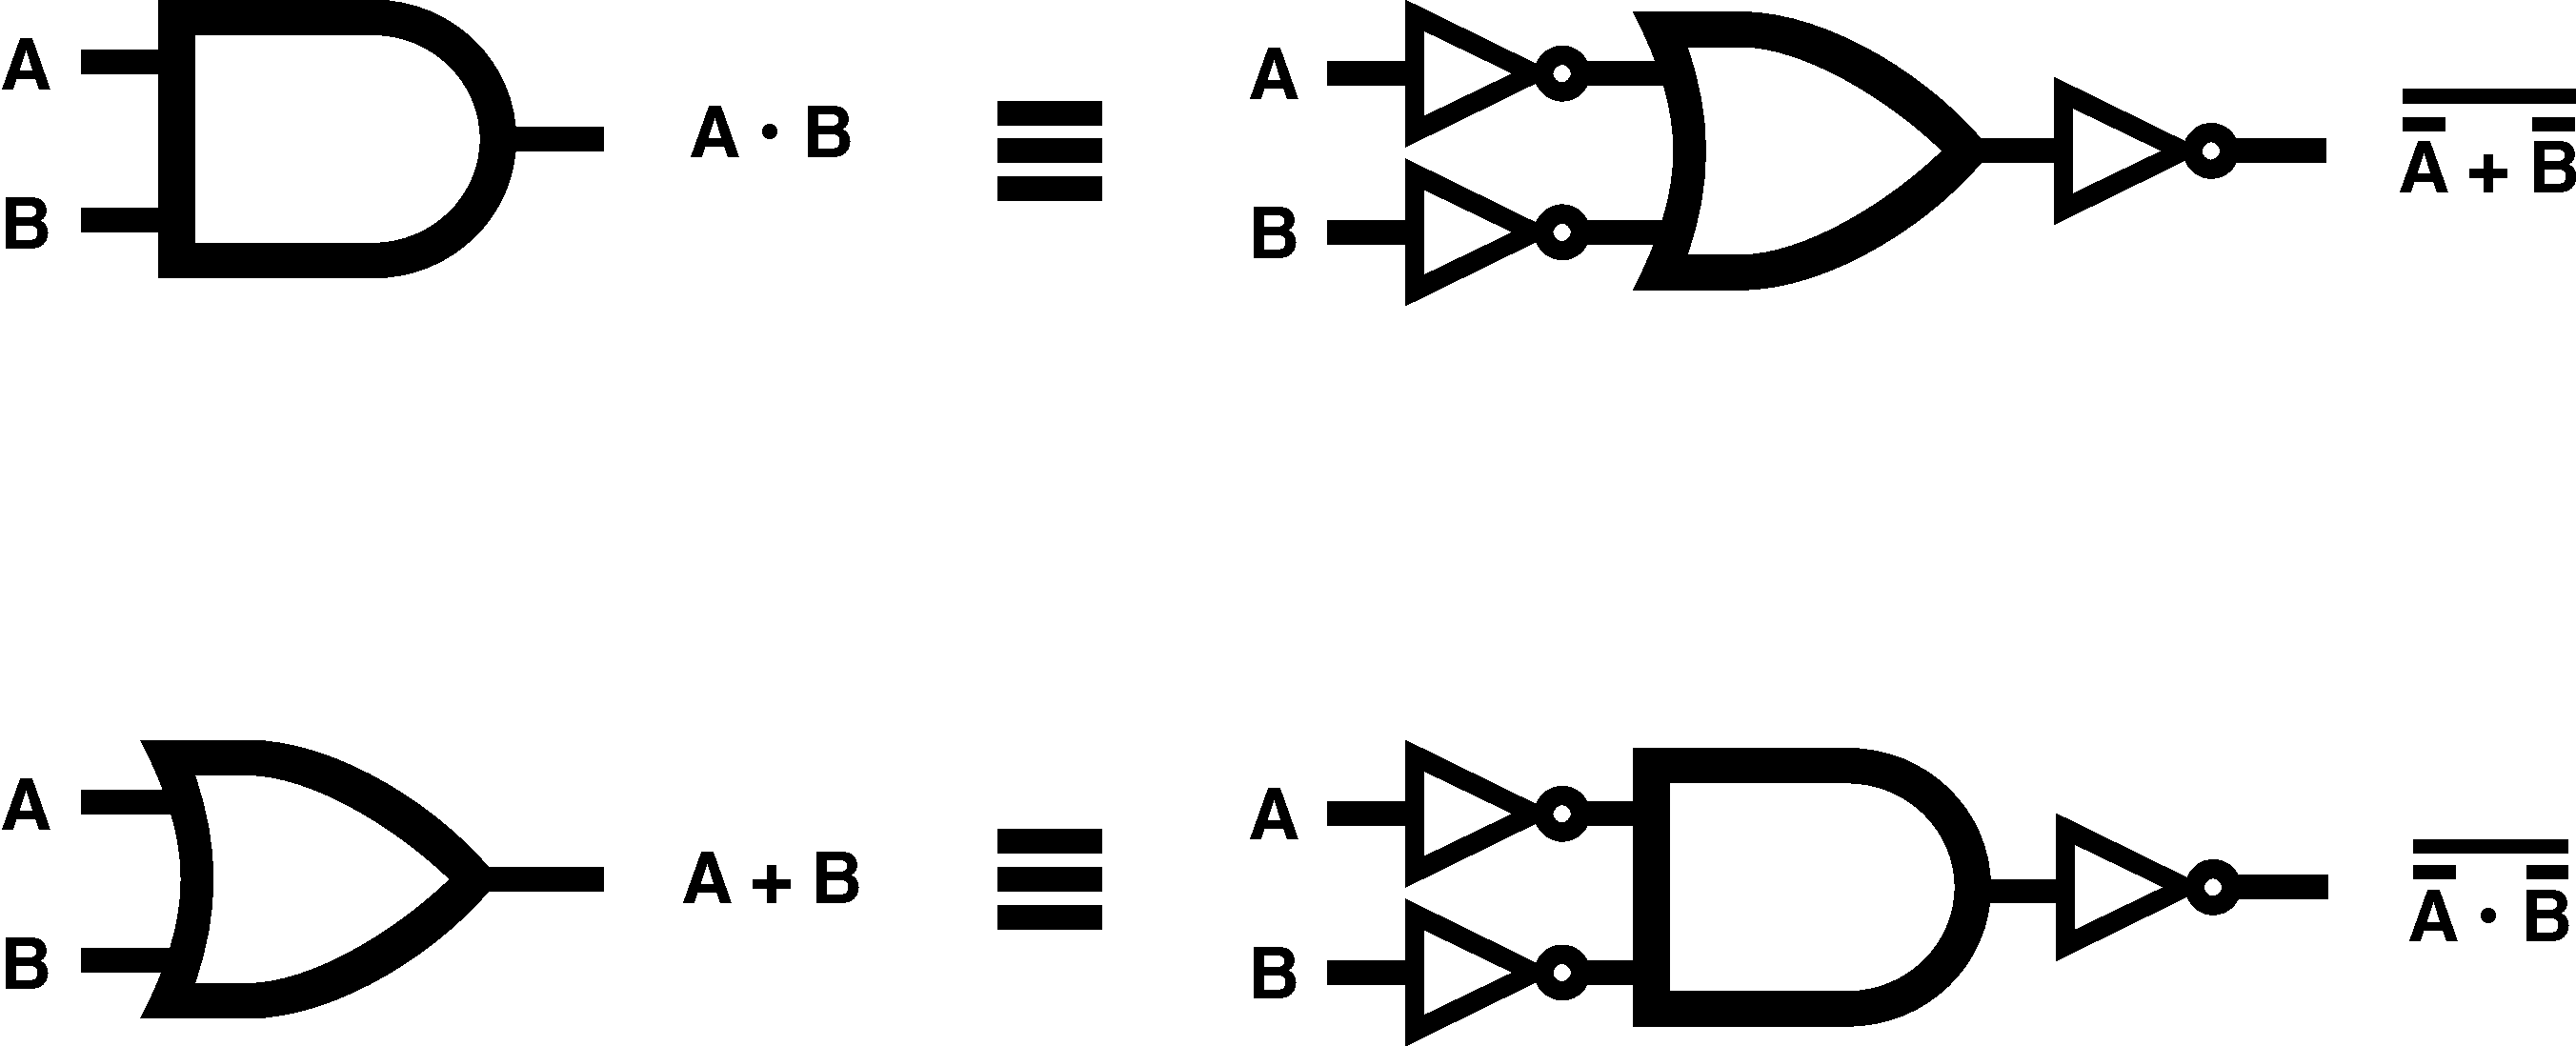
\includegraphics[width=0.8\linewidth]{images/2_elettronica/demorgan_2.pdf}
%		\caption{}
	\end{figure}
\end{frame}


\begin{frame}
	\frametitle{Esercizi sulle leggi di De Morgan: \#1}

	\begin{block}{Riscrivere la proposizione logica $\overline{X} + Y$ (che utilizza \textit{not} e \textit{or}) applicando le leggi di De Morgan, utilizzando solo le porte logiche \textit{not} e \textit{and}.}
		
		Ricordando che $A + B = \overline{\overline {A} \cdot \overline {B}}$\\
		\pause
		Focalizzandosi sulla parte sinistra dell'equazione la proposizione logica di partenza può essere vista come $A = \overline {X}$ e $B = Y$ del caso.\\
		\pause
		Quindi prendiamo la proposizione $\overline{\overline {A} \cdot \overline {B}}$ e sostituiamo i nostri $A$ e $B$.\\~\\
		\pause
		
		$$\overline{\overline {A} \cdot \overline {B}} = \overline{\overline {\overline {X}} \cdot \overline {Y}} = \overline{X \cdot \overline {Y}}$$
		\pause
		$$Quindi$$
		
		$$\overline{X} + Y = \overline{X \cdot \overline {Y}}$$ 
		
		
			
	\end{block}
	
\end{frame}


\begin{frame}
	\frametitle{Esercizi sulle leggi di De Morgan: \#2}

	\begin{block}{Rappresentare graficamente i due circuiti logici equivalenti del punto precedente, ovvero il circuito per $\overline{X} + Y$ e il circuito per $\overline{X \cdot \overline {Y}}$}
		\vspace{1em}
		\pause
		\begin{figure}[!htbp]
			\centering 
			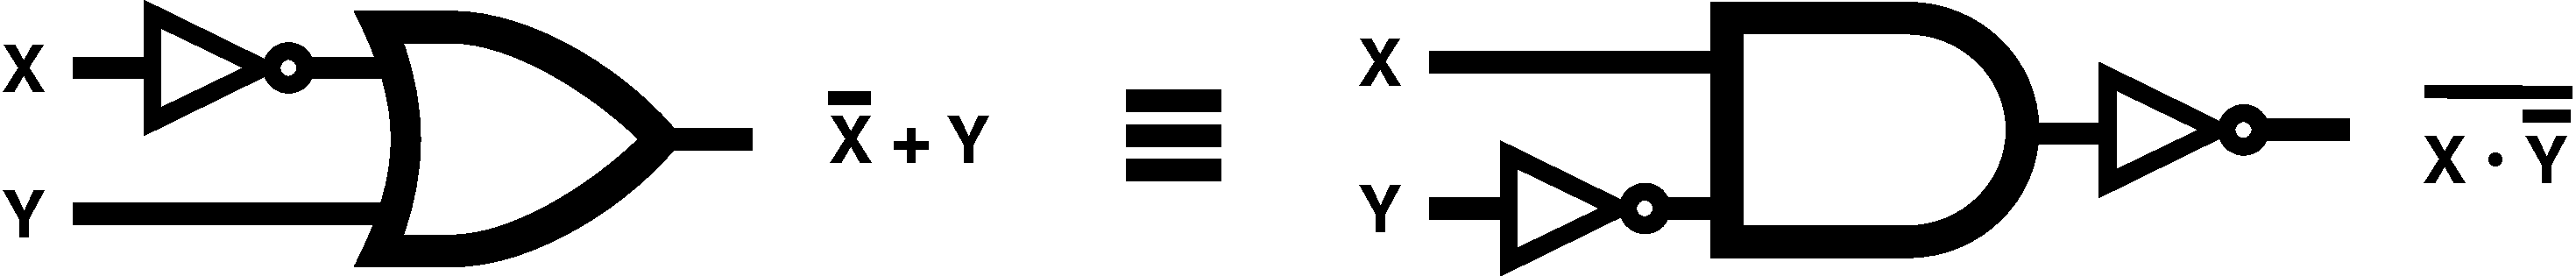
\includegraphics[width=0.8\linewidth]{images/2_elettronica/demorgan_ex.pdf}
	%		\caption{}
		\end{figure}
			
	\end{block}
	
\end{frame}



\begin{frame}
	\frametitle{Esercizi sulle leggi di De Morgan: \#3}

	\begin{block}{Compilare la tabella di verità della proposizione $\overline{X} + Y$}
	
		\begin{scriptsize}
			\begin{columns}
				\column{0.3\linewidth}
				\begin{table}[]
				\begin{tabular}{|
				>{\columncolor[HTML]{C0C0C0}}c |
				>{\columncolor[HTML]{C0C0C0}}c |c|}
				\hline
				\cellcolor[HTML]{EFEFEF}\textbf{$\pmb{X}$} & \cellcolor[HTML]{EFEFEF}\textbf{$\pmb{Y}$} & \cellcolor[HTML]{EFEFEF}$\pmb{\pmb{\overline{X} + Y}}$ \\ \hline
				0                                  & 0                         &                                     \\ \hline
				0                                  & 1                         &                                     \\ \hline
				1                                  & 0                         &                                     \\ \hline
				1                                  & 1                         &                                    \\ \hline
				\end{tabular}
				\end{table}
				\pause
				
				\column{0.35\linewidth}
				\begin{table}[]
				\begin{tabular}{|
				>{\columncolor[HTML]{C0C0C0}}c |
				>{\columncolor[HTML]{C0C0C0}}c |
				>{\columncolor[HTML]{C0C0C0}}c |c|}
				\hline
				\cellcolor[HTML]{EFEFEF}\textbf{$\pmb{X}$} & \cellcolor[HTML]{EFEFEF}\textbf{$\pmb{Y}$} & \cellcolor[HTML]{EFEFEF}$\pmb{\overline{X}}$ & \cellcolor[HTML]{EFEFEF}$\pmb{\pmb{\overline{X} + Y}}$ \\ \hline
				0                                  & 0                                  & 1                                  &                                     \\ \hline
				0                                  & 1                                  & 1                                  &                                     \\ \hline
				1                                  & 0                                  & 0                                  &                                     \\ \hline
				1                                  & 1                                  & 0                                  &                                     \\ \hline
				\end{tabular}
				\end{table}
				\pause
				
				\column{0.35\linewidth}
				\begin{table}[]
				\begin{tabular}{|
				>{\columncolor[HTML]{C0C0C0}}c |
				>{\columncolor[HTML]{C0C0C0}}c |
				>{\columncolor[HTML]{C0C0C0}}c |c|}
				\hline
				\cellcolor[HTML]{EFEFEF}\textbf{$\pmb{X}$} & \cellcolor[HTML]{EFEFEF}\textbf{$\pmb{Y}$} & \cellcolor[HTML]{EFEFEF}$\pmb{\overline{X}}$ & \cellcolor[HTML]{EFEFEF}$\pmb{\pmb{\overline{X} + Y}}$ \\ \hline
				0                                  & 0                                  & 1                                  & 1                                    \\ \hline
				0                                  & 1                                  & 1                                  & 1                                    \\ \hline
				1                                  & 0                                  & 0                                  & 0                                    \\ \hline
				1                                  & 1                                  & 0                                  & 1                                    \\ \hline
				\end{tabular}
				\end{table}
				
			\end{columns}
		\end{scriptsize}
		
		\pause
		Ricordiamo che la tabella di verità ottenuta sarà identica a quella di $\overline{X \cdot \overline {Y}}$ in quanto sono circuiti equivalenti. La tabella di verità di $\overline{X} + Y$ quindi è:
		
		\begin{scriptsize}
		
			\begin{columns}
				\column{0.4\linewidth}
				\begin{table}[]
				\begin{tabular}{|
				>{\columncolor[HTML]{C0C0C0}}c |
				>{\columncolor[HTML]{C0C0C0}}c |c|}
				\hline
				\cellcolor[HTML]{EFEFEF}\textbf{$\pmb{X}$} & \cellcolor[HTML]{EFEFEF}\textbf{$\pmb{Y}$} & \cellcolor[HTML]{EFEFEF}$\pmb{\pmb{\overline{X} + Y}}$ \\ \hline
				0                                  & 0                         & 1                                    \\ \hline
				0                                  & 1                         & 1                                    \\ \hline
				1                                  & 0                         & 0                                    \\ \hline
				1                                  & 1                         & 1                                   \\ \hline
				\end{tabular}
				\end{table}
				
				\column{0.1\linewidth}
				\begin{huge}
					\begin{center}
						$\equiv$
					\end{center}
				\end{huge}
				
				
				\column{0.4\linewidth}
				\begin{table}[]
				\begin{tabular}{|
				>{\columncolor[HTML]{C0C0C0}}c |
				>{\columncolor[HTML]{C0C0C0}}c |c|}
				\hline
				\cellcolor[HTML]{EFEFEF}\textbf{$\pmb{X}$} & \cellcolor[HTML]{EFEFEF}\textbf{$\pmb{Y}$} & \cellcolor[HTML]{EFEFEF}$\pmb{\overline{X \cdot \overline {Y}}}$ \\ \hline
				0                                  & 0                         & 1                                    \\ \hline
				0                                  & 1                         & 1                                    \\ \hline
				1                                  & 0                         & 0                                    \\ \hline
				1                                  & 1                         & 1                                   \\ \hline
				\end{tabular}
				\end{table}				
			\end{columns}
			
			
		\end{scriptsize}
			
	\end{block}
	
\end{frame}


\subsection[I generatori di segnali]{I generatori di segnali}
\begin{frame}
	\frametitle{I generatori di segnali}
	
	\begin{block}{I generatori di segnali}
		I \textbf{generatori di segnali} sono componenti elettronici che producono segnali elettrici di varie frequenze e forme d'onda per sincronizzare e coordinare le operazioni all'interno di un computer.
	\end{block}
	
	\begin{figure}[!htbp]
		\centering 
		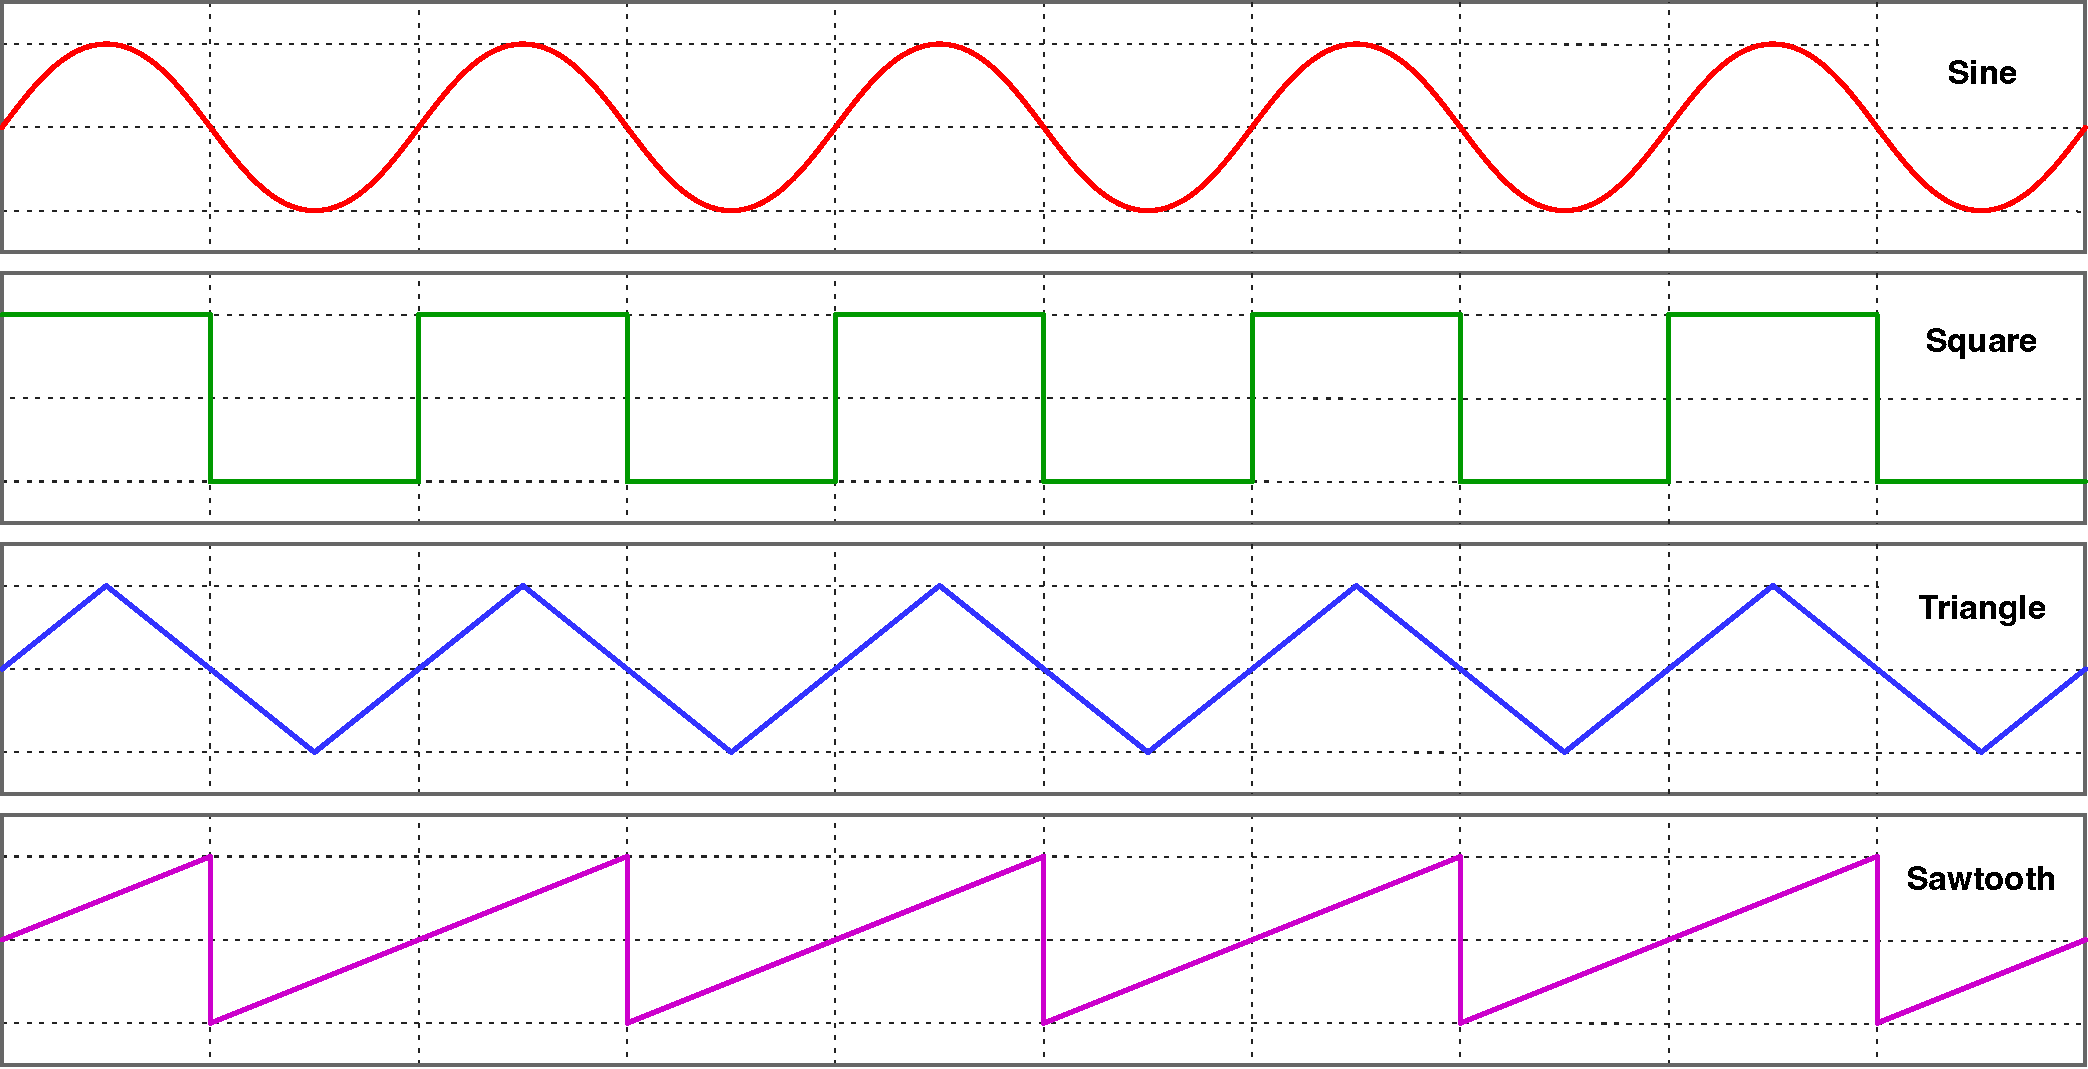
\includegraphics[width=0.65\linewidth]{images/2_elettronica/waveforms.pdf}
		\caption{Forme d'onda sinusoidale, quadrata, triangolare e a dente di sega}
		\label{fig:electronics_waveforms}
	\end{figure}
\end{frame}


\subsection[Il clock]{Il clock}
\begin{frame}
	\frametitle{Il clock}
	
	\begin{block}{Il clock}
		Il \textbf{clock} è un generatore di segnale, generalmente realizzato utilizzando un \textit{oscillatore al quarzo}, che viene utilizzato per \textit{sincronizzare} e \textit{coordinare} le operazioni all'interno di un computer, produce un \textbf{segnale periodico} con forma di \textbf{onda quadra}.
	\end{block}
	
	\begin{columns}
		\column{0.38\linewidth}
		\begin{itemize}
			\item $\mathrm{T} \rightarrow $ periodo o ciclo,\\
			unità di misura in\\
			$s$ (secondi)\\~\\
			\item $f = \frac{1}{\mathrm{T}} \rightarrow$ frequenza,\\
			unità di misura in $Hz = \frac{1}{s}$ (hertz)
		\end{itemize}
		
		\column{0.62\linewidth}
		\begin{figure}[!htbp]
			\centering 
			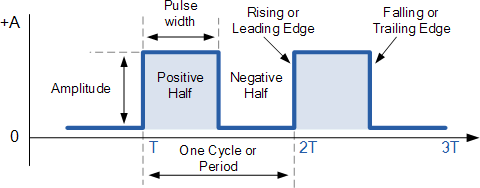
\includegraphics[width=1.0\linewidth]{images/2_elettronica/clock.png}
			\caption{Il ciclo di clock}
		\end{figure}
		
	\end{columns}
	
\end{frame}


\subsubsection[Il periodo $\mathrm{T}$]{Il periodo $\mathrm{T}$}
\begin{frame}
	\frametitle{Il clock: il periodo $\mathrm{T}$}
	
	\begin{block}{Il periodo $\mathrm{T}$}
		Il periodo $\mathrm{T}$ di un'onda è il tempo impiegato per eseguire un'oscillazione completa.\\
		Nel caso del clock viene detto \textbf{periodo di clock} oppure \textbf{tempo di ciclo} e corrisponde ad il tempo in secondi ($s$) che intercorre tra un fronte di salita e quello successivo (o tra un fronte di discesa e quello successivo).
	\end{block}
	
	\begin{figure}[!htbp]
		\centering 
		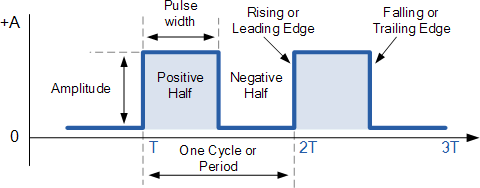
\includegraphics[width=0.78\linewidth]{images/2_elettronica/clock.png}
%		\caption{Il ciclo di clock}
	\end{figure}
	
\end{frame}


\subsubsection[La frequenza $f$]{La frequenza $f$}
\begin{frame}
	\frametitle{Il clock: la frequenza $f$}
	
	\begin{block}{La frequenza $f$}
		La \textbf{frequenza} $f$ di un'onda è il numero di oscillazioni complete al secondo.\\
		Questa si misura in Hertz ($Hz$) ovvero in \textbf{oscillazioni al secondo}.\\
		È uno dei parametri più importanti per misurare le prestazioni di un processore.\\
		A volte come sinonimo di frequenza di clock si può trovare utilizzato il termine velocità di clock.
	\end{block}
	
	
	\begin{figure}[!htbp]
		\centering 
		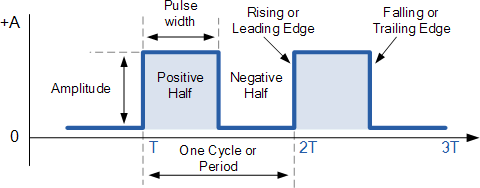
\includegraphics[width=0.78\linewidth]{images/2_elettronica/clock.png}
%		\caption{Il ciclo di clock}
	\end{figure}
	
\end{frame}


\subsubsection[La relazione tra $\mathrm{T}$ e $f$: $f = \frac{1}{\mathrm{T}}$ e $\mathrm{T} = \frac{1}{f}$]{La relazione tra $\mathrm{T}$ e $f$: $f = \frac{1}{\mathrm{T}}$ e $\mathrm{T} = \frac{1}{f}$}
\begin{frame}
	\frametitle{Il clock: la relazione tra $\mathrm{T}$ e $f$ $\rightarrow$ $f = \frac{1}{\mathrm{T}}$ e $\mathrm{T} = \frac{1}{f}$}
		
	\begin{figure}[!htbp]
		\centering 
		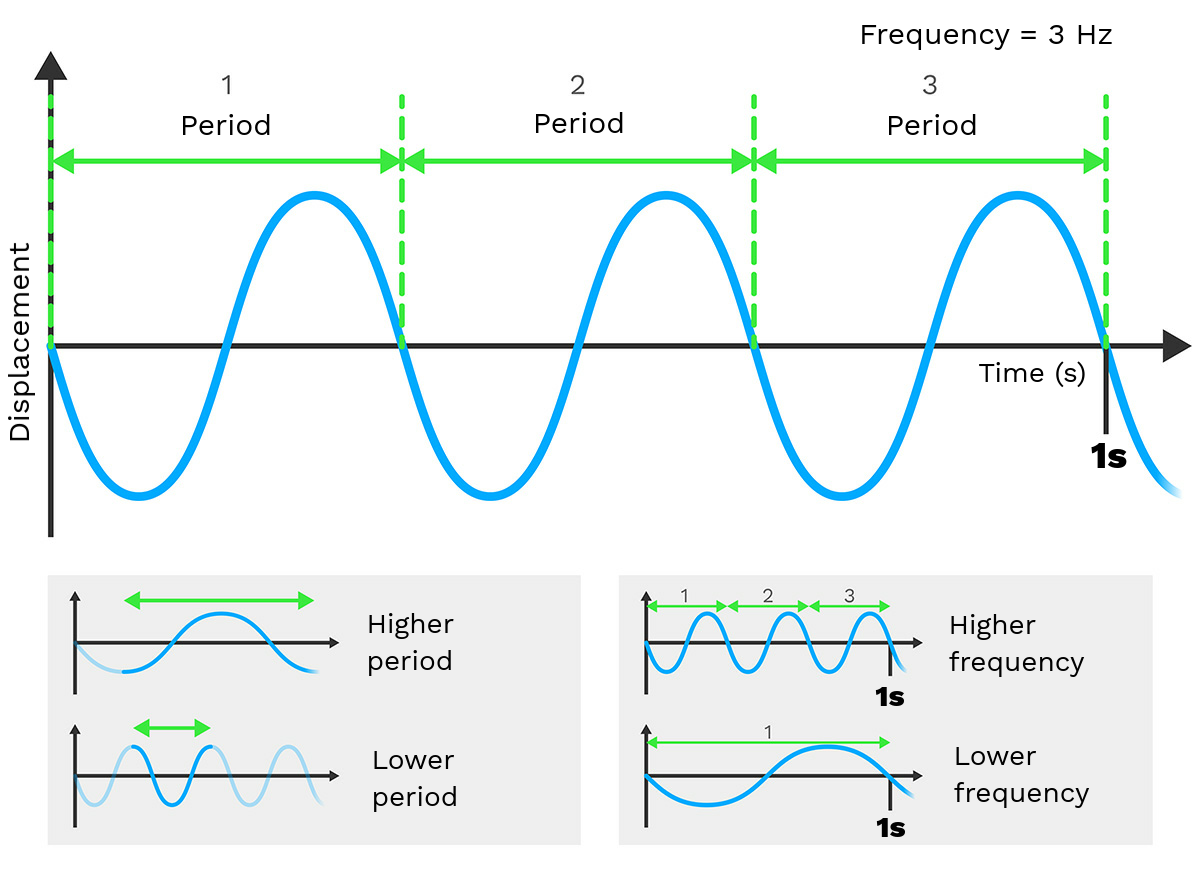
\includegraphics[width=0.82\linewidth]{images/2_elettronica/period_frequency.png}
		\caption{La relazione che intercorre tra periodo e frequenza}
		\label{fig:electronics_period_frequency}
	\end{figure}
\end{frame}


\begin{frame}
	\frametitle{Esercizi sulla relazione tra $\mathrm{T}$ e $f$:}
	
	\begin{block}{Esercizio 1: calcola il periodo $\mathrm{T}$ conoscendo la frequenza $f$}
		Un \textbf{processore} con \textbf{frequenza di clock} (o velocità di clock) di \textbf{4.0 $\pmb{GHz}$} (giga$Hz$) esegue 4 miliardi di cicli completi al secondo.\\
		In passato le CPU erano molto più lente di oggi e la frequenza di clock era misurata in $MHz$ (mega$Hz$) ovvero milioni di cicli completi al secondo.\\
		\textbf{Quanto dura il periodo di clock $\pmb{\mathrm{T}}$ per il suddetto processore?}\\~\\
		\pause
		Ricordando che la relazione tra $\mathrm{T}$ e $f$ è del tipo $\mathrm{T} = \frac{1}{f}$ possiamo calcolare la durata del periodo di clock $\mathrm{T}$ conoscendo la frequenza $f$ come segue:\\~\\
		\pause
		$\quad\,\, \mathrm{T} = \frac{1}{f} = \frac{1}{4 GHz} = \frac{1}{4 \cdot 10^9 Hz} = \frac{1}{4 \cdot 10^9 1/s} = \frac{1}{4 \cdot 10^9 s^{-1}} = \frac{1}{4} \cdot 10^{-9} s = 0.25ns$\\ \vspace{0.4em}
		\pause
		$\qquad\qquad\qquad\qquad\qquad\qquad\qquad$	quindi:\\ \vspace{0.4em}
%		\begin{center}
%			quindi:
%		\end{center}
		$\qquad\qquad\qquad\qquad \mathrm{T} = 0.25ns = 250 ps = 250$ picosecondi
	\end{block}
	
\end{frame}


\begin{frame}
	\frametitle{Esercizi sulla relazione tra $\mathrm{T}$ e $f$:}
	
	\begin{block}{Esercizio 2: calcola la frequenza $f$ conoscendo il periodo $\mathrm{T}$}
		\textbf{Che frequenza di clock ha un processore con periodo di clock di 200$\pmb{ps}$ (picosecondi)?}\\~\\
		\pause
		Ricordando che la relazione tra $f$ e $\mathrm{T}$ è del tipo $f = \frac{1}{\mathrm{T}}$ possiamo calcolare la frequenza di clock $f$ conoscendo la durata del periodo di clock $\mathrm{T}$ come segue:\\~\\
		\pause
		$\qquad f = \frac{1}{\mathrm{T}} = \frac{1}{200 ps} = \frac{1}{200 \cdot 10^{-12} s} = \frac{1}{0.2 \cdot 10^{-9} s} = \frac{1}{0.2} \cdot \dot 10^9 s^{-1} = 5 GHz$
		\pause
		\begin{center}
			quindi:
		\end{center}
		$\qquad\qquad\qquad\qquad\qquad\;\; f = 5 GHz = 5 gigahertz$
	\end{block}
	
\end{frame}


